\section{Question}

\large{\textbf{We now turn to sequence comparison and alignment. You are given the following coding sequence fragments. They encode a homologous proteins in different species, sequence 2 is human (1 extra mark if you can give the gene name and the most likely species for the other sequences). The sequences are aligned to the correct reading frame:}}

\medskip

\texttt{1. CTGAAGCGGGAGGCTGAGACGCTGCGGGAGCGGGAGGGC}

\texttt{2. CTCAAGCGTGAGGCCGAGACCCTACGGGAGCGGGAAGGC}

\texttt{3. GAAGAGCTGAAGAGAGAGGCTGACAATTTAAAGGACAGA}

\texttt{4. AACGAGGAGCTCAAGCGAGAAGCTGATACGCTGAAGGAC}

\medskip

% - - - - - - - - - - - - - - - - - - - - - - - - - - -

\subsection{Sequences 1 and 2 differ slightly. How does the resulting protein differ? Could this have functional implications?}

The resulting protein does not differ, it is the same: \texttt{LKREAETLREREG}. Since the encoded amino acids do not change, the protein has exactly the same functionality.

One might theorise that this amino acid encoding redundancy is a biological safeguard for small mutations not to change the functionality of a protein.

\medskip

% - - - - - - - - - - - - - - - - - - - - - - - - - - -

\subsection{Now use the Needleman-Wunsch algorithm to compare sequence 1 to sequences 3 and 4. Use the scoring: match +2, mismatch -1, indel -1. Perform at least one of these on paper (or both if you wish). On paper, use the first three codons only.}

\begin{figure}[ht]
    \centering
    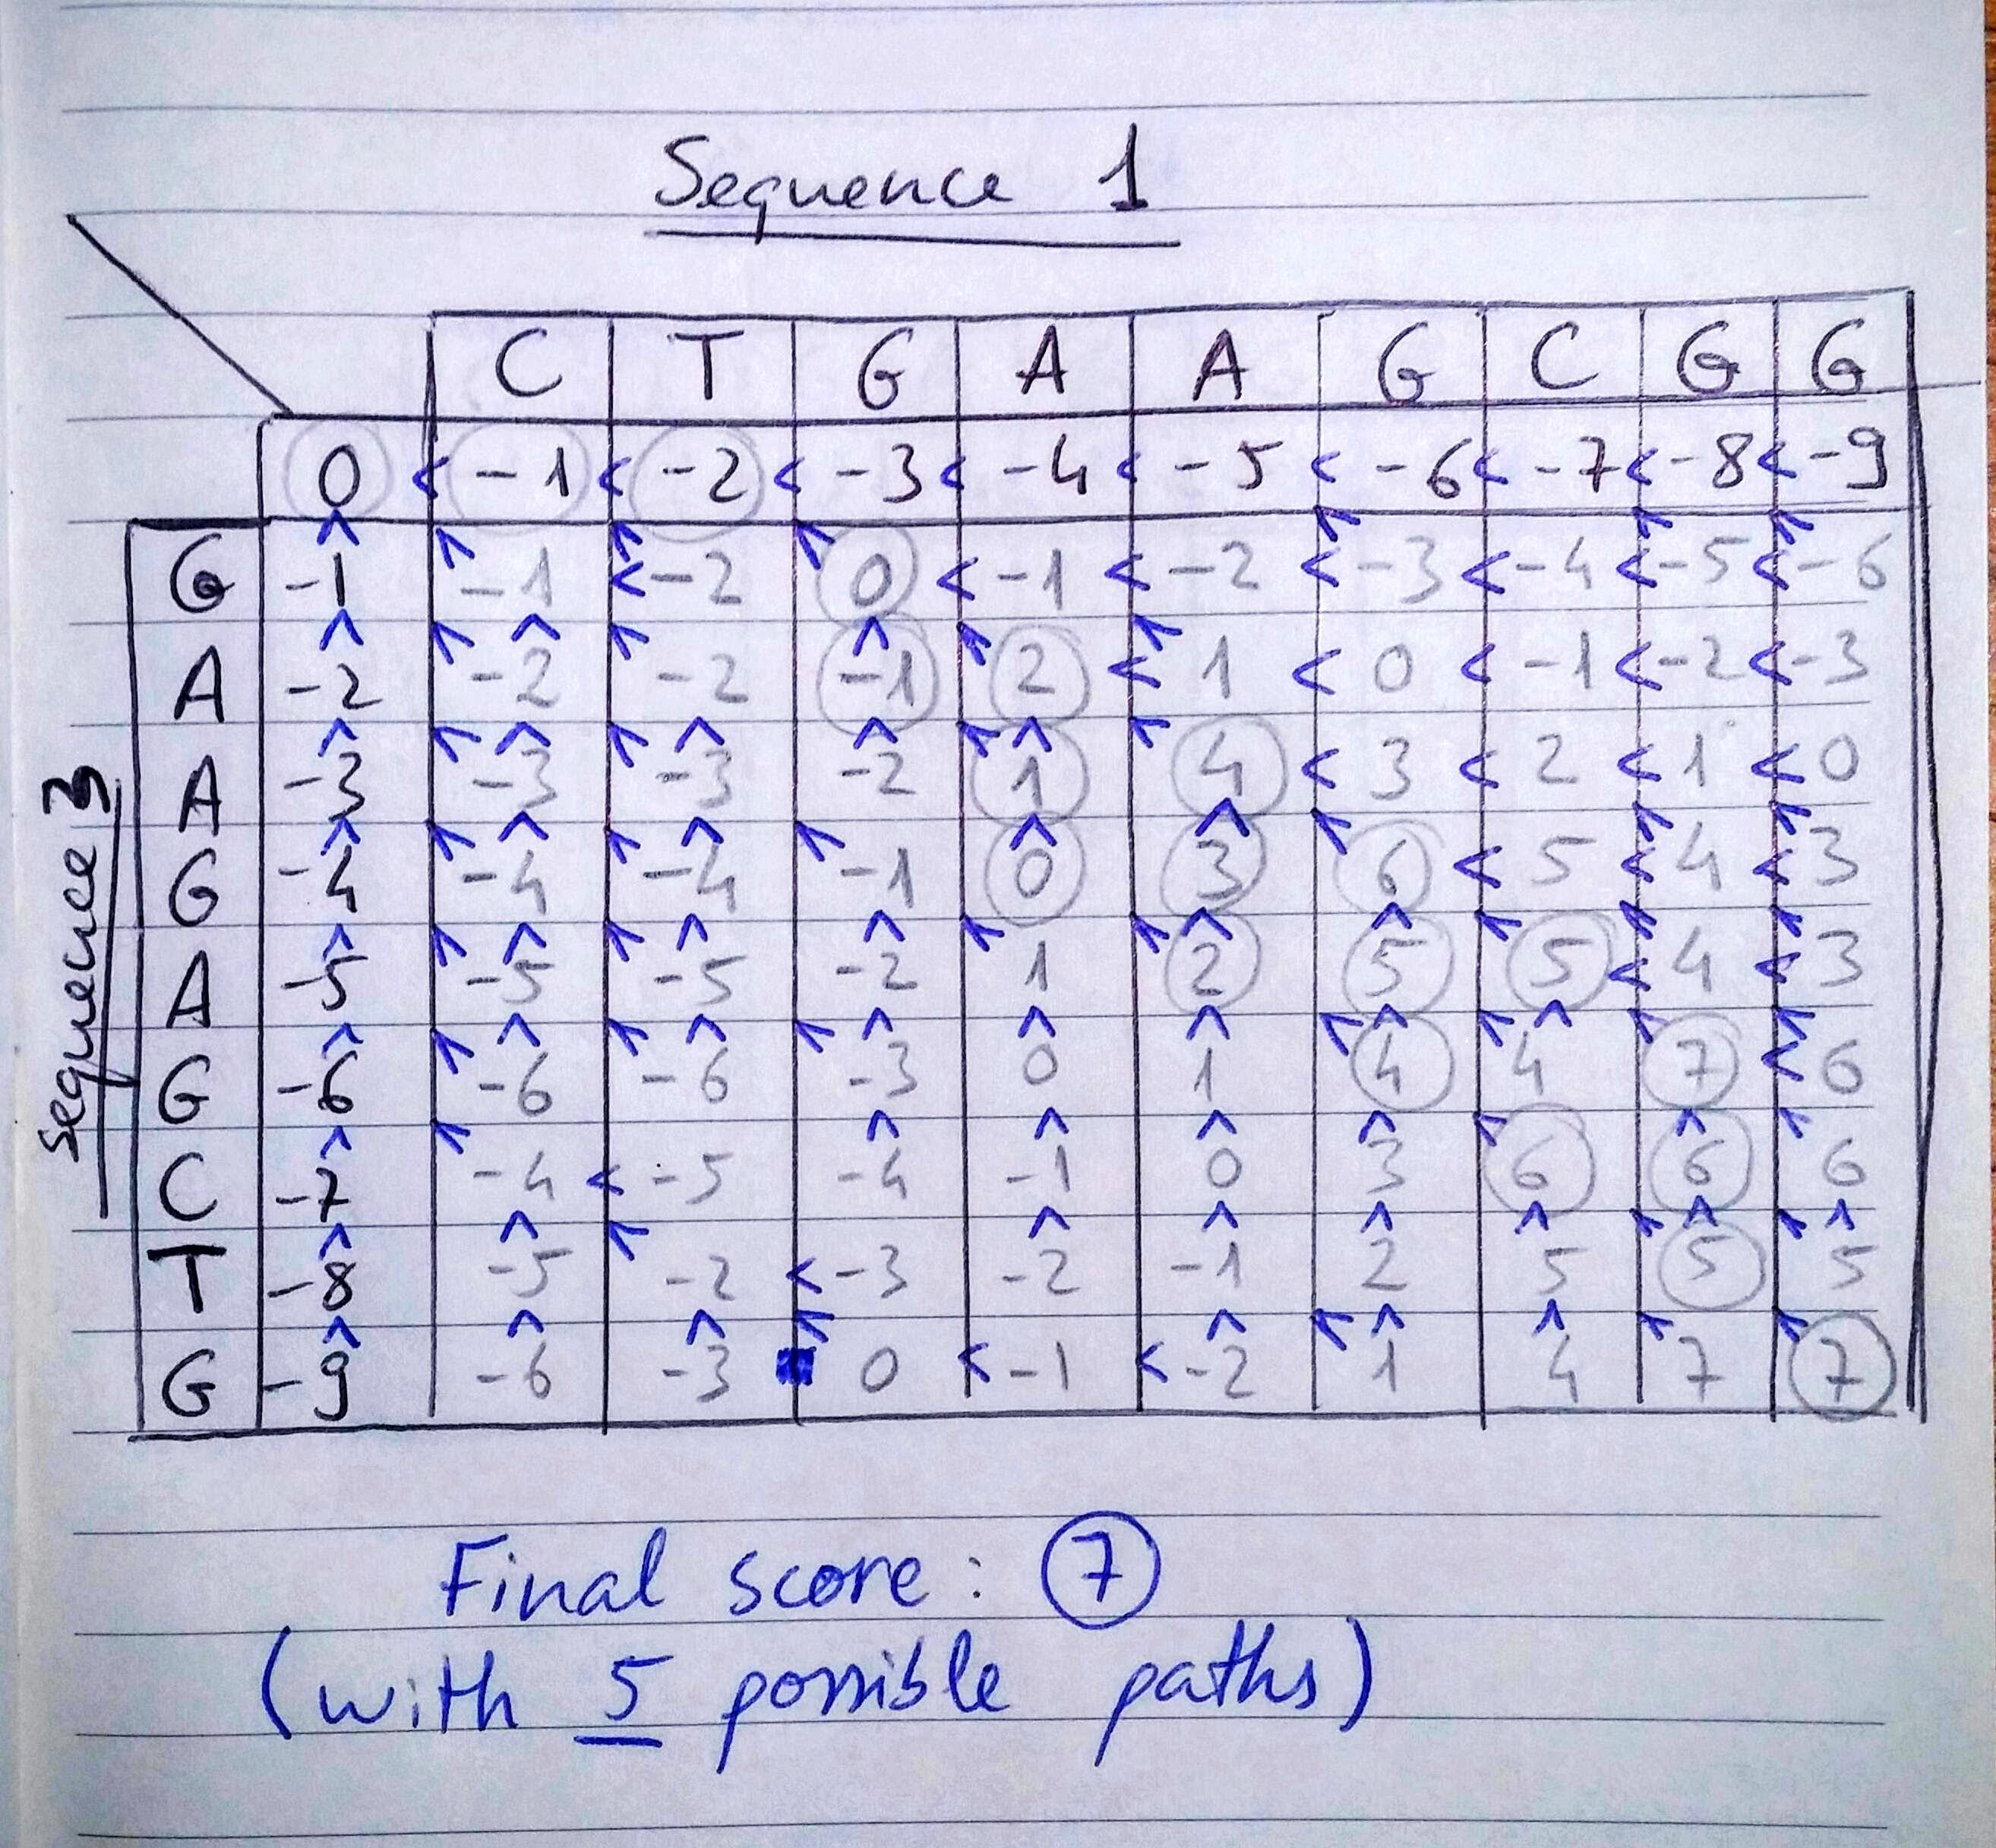
\includegraphics[width=0.6\linewidth]{res/needleman-wunsch-seq1-seq3.jpg}
    \caption{Needleman-Wunsch algorithm result on sequence 1 and 3.}
    \label{fig:needleman-wunsch-seq1-seq3}
\end{figure}

\begin{figure}[ht]
    \centering
    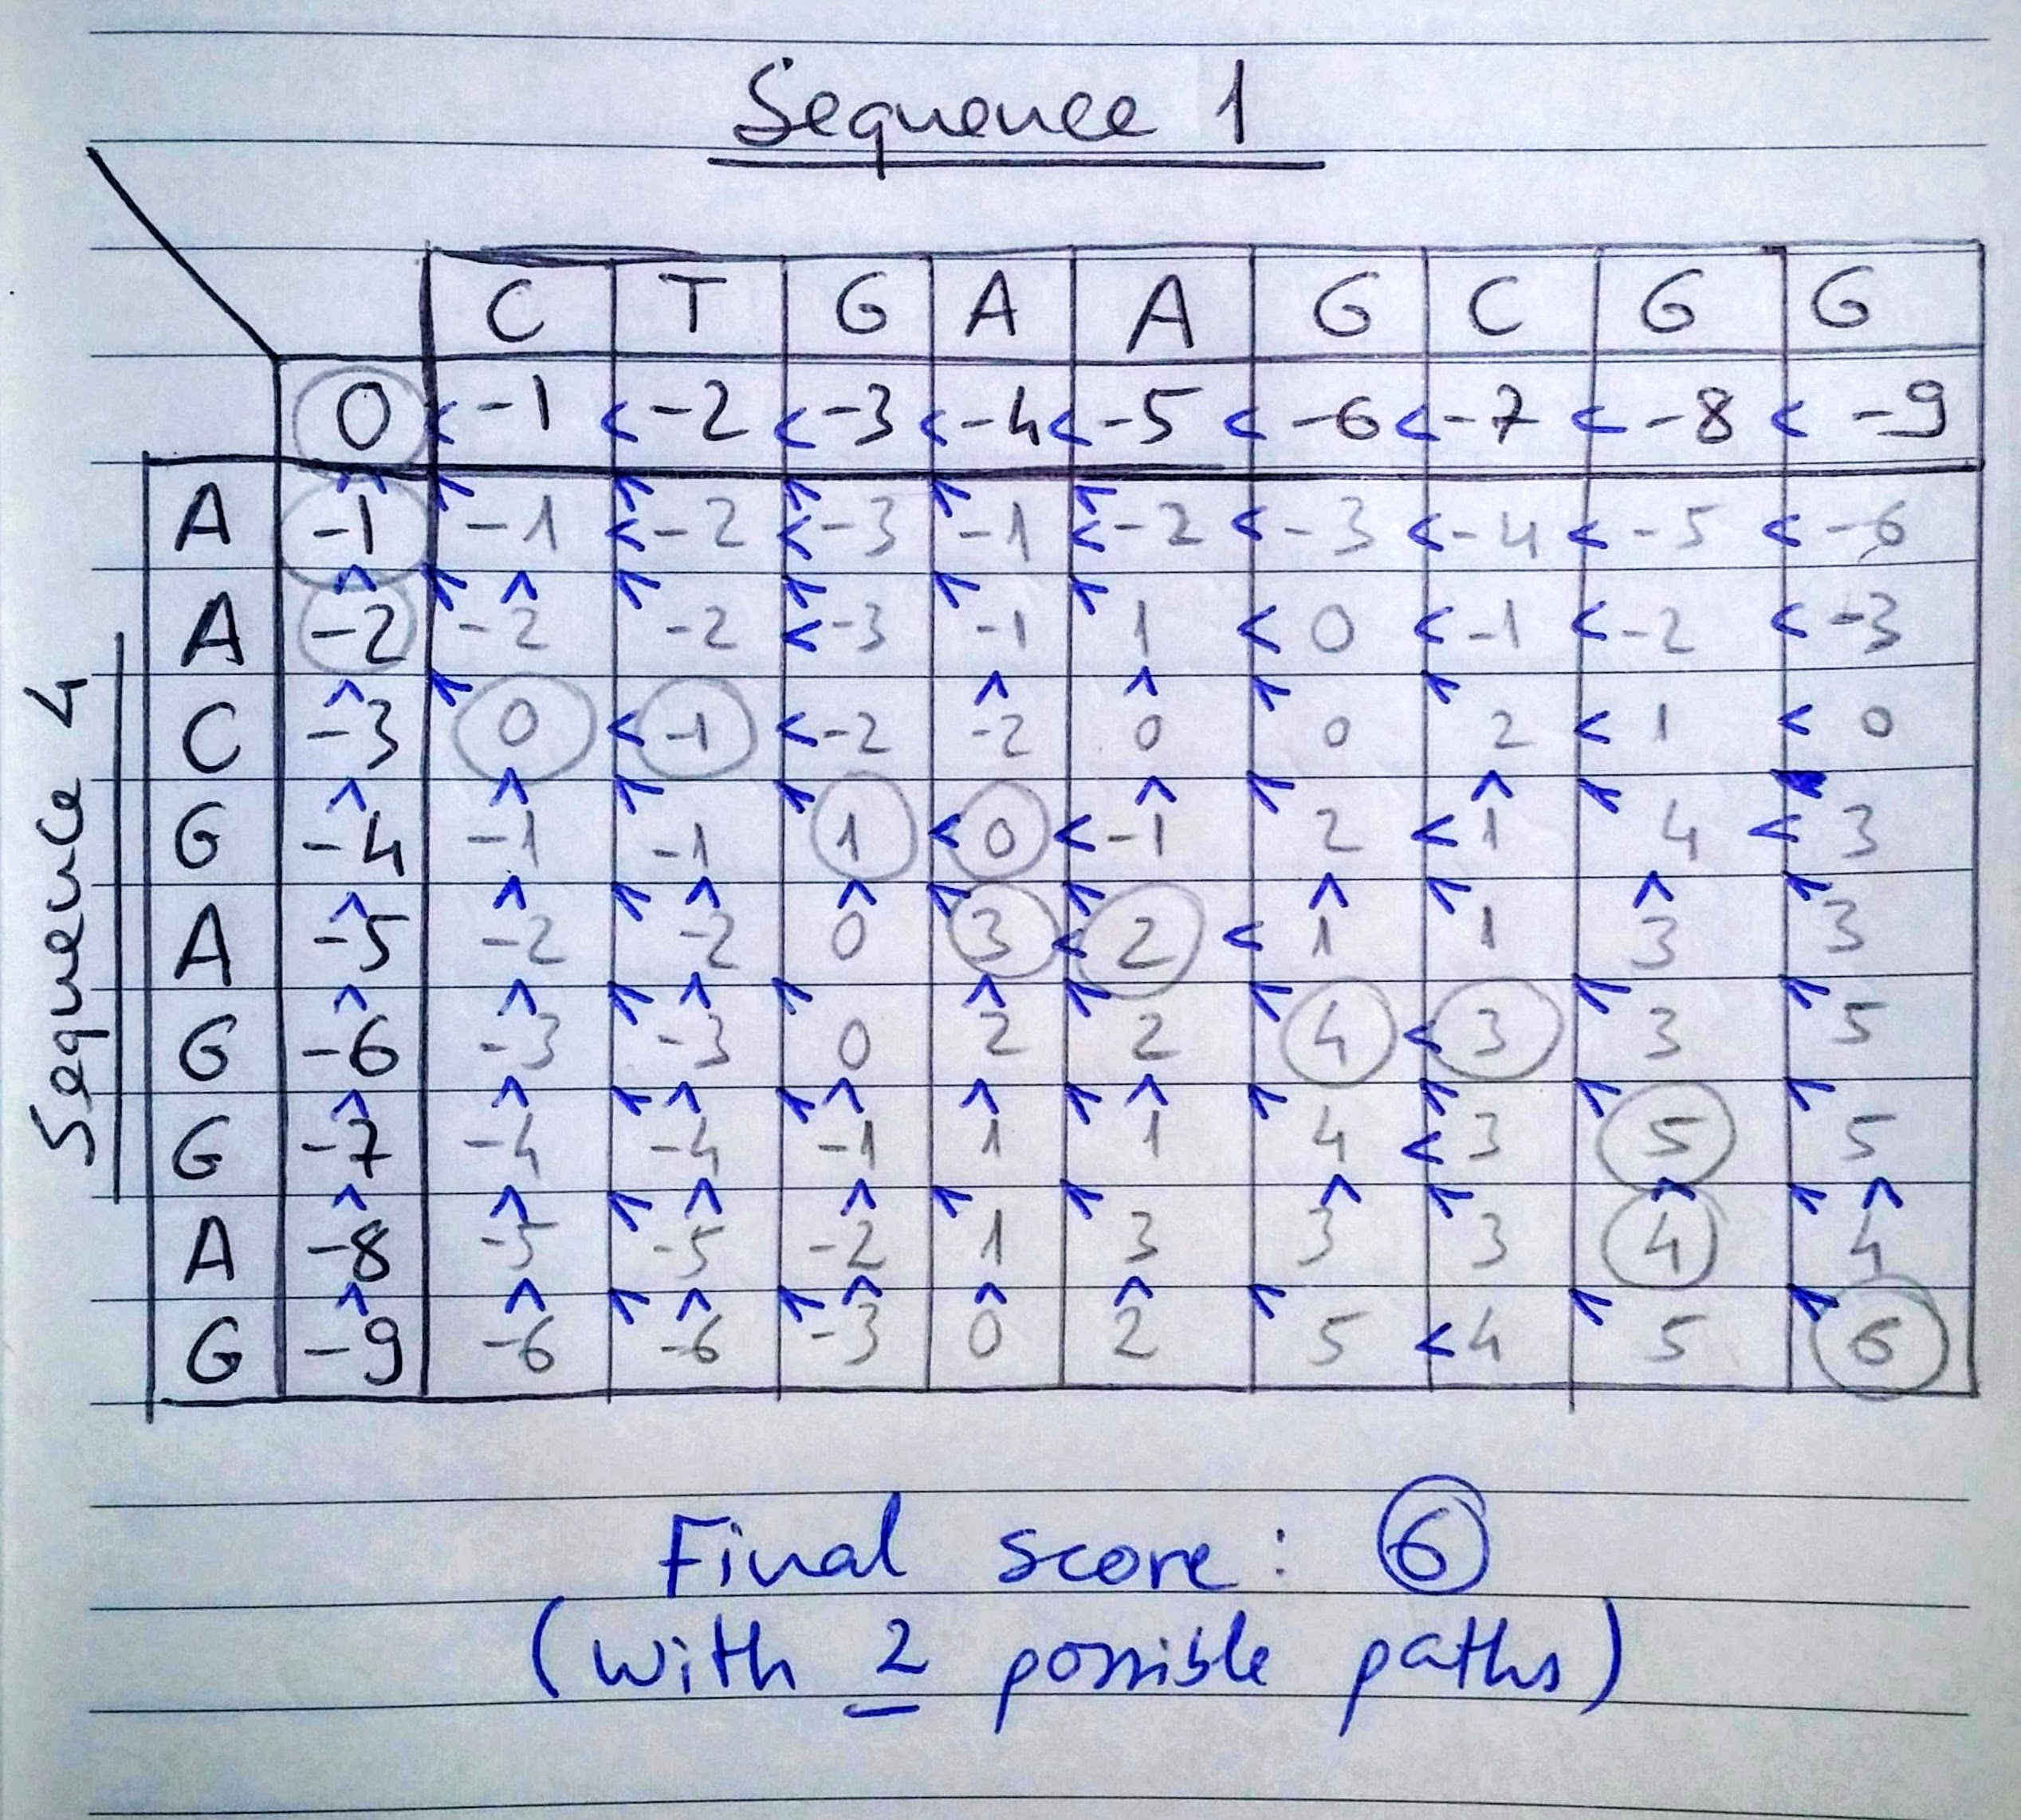
\includegraphics[width=0.6\linewidth]{res/needleman-wunsch-seq1-seq4.jpg}
    \caption{Needleman-Wunsch algorithm result on sequence 1 and 4.}
    \label{fig:needleman-wunsch-seq1-seq4}
\end{figure}

\clearpage

% - - - - - - - - - - - - - - - - - - - - - - - - - - -

\subsection{Comparing the bare sequences, what can you conclude about the relatedness of the species?}

TODO

\medskip

% - - - - - - - - - - - - - - - - - - - - - - - - - - -

\subsection{Extra mark}

TODO

\begin{center}
	\begin{tabu} to 0.8\textwidth{ | X[c] | X[c] | X[c] | }
		\hline
		Sequence & Gene name & Species \\
		\hline
		1 & ? & ? \\
		2 & ? & human \\
		3 & ? & ? \\
		4 & ? & ? \\
		\hline
	\end{tabu}
\end{center}

\newpage
